Looking at system designs towards Exascale~\cite{top500}, one will not hesitate to predict that future systems will be based on more powerful compute nodes rather than more nodes~\cite{Shalf:exascaleChallenges}.  
An inevitable consequence of this design trend is that node architecture will be more complex.
Indeed, it is common to see traditional multi-core CPUs augmented with multiple high-end graphics cards such as NVIDIA's GPUs or Intel's first generation Xeon Phi coprocessors (KNC).
Other accelerator architectures such as FPGA and Automata Processor (digital) and Neuromorphic Processor (non-digital) have been gaining more traction.
Heterogeneous programming is challenging~\cite{exascaleRoadMap}, mainly because realizing high performance and scalability on accelerators is difficult.
Even when an application performs well on accelerators, load imbalance arises since CPUs and accelerators run at different rates.
Beside the problems above, the programmer has to handle the communication between CPUs and accelerators, e.g. via PCIe, NVLink, etc.
% (see Fig.~\ref{fig:sysArch}).

To avoid these problems, compute nodes can be based on stand-alone many-core processors such as the Intel's second generation Xeon Phi processor (KNL).
However, applications consisting of both task and data parallelism may not be well-suited to such homogeneous designs.
In addition, realizing expected performance on stand-alone many-core processors also requires expert programming skills
to manually manage data movement and locality.
In this paper, we focus on tackling challenges associated with the heterogeneous CPU-GPU node design, though our solution can also support the homogeneous case and be extended to support other accelerator architectures.

%\begin{figure}[htb]
%\centering
%\begin{subfigure}[b]{0.22\textwidth}
%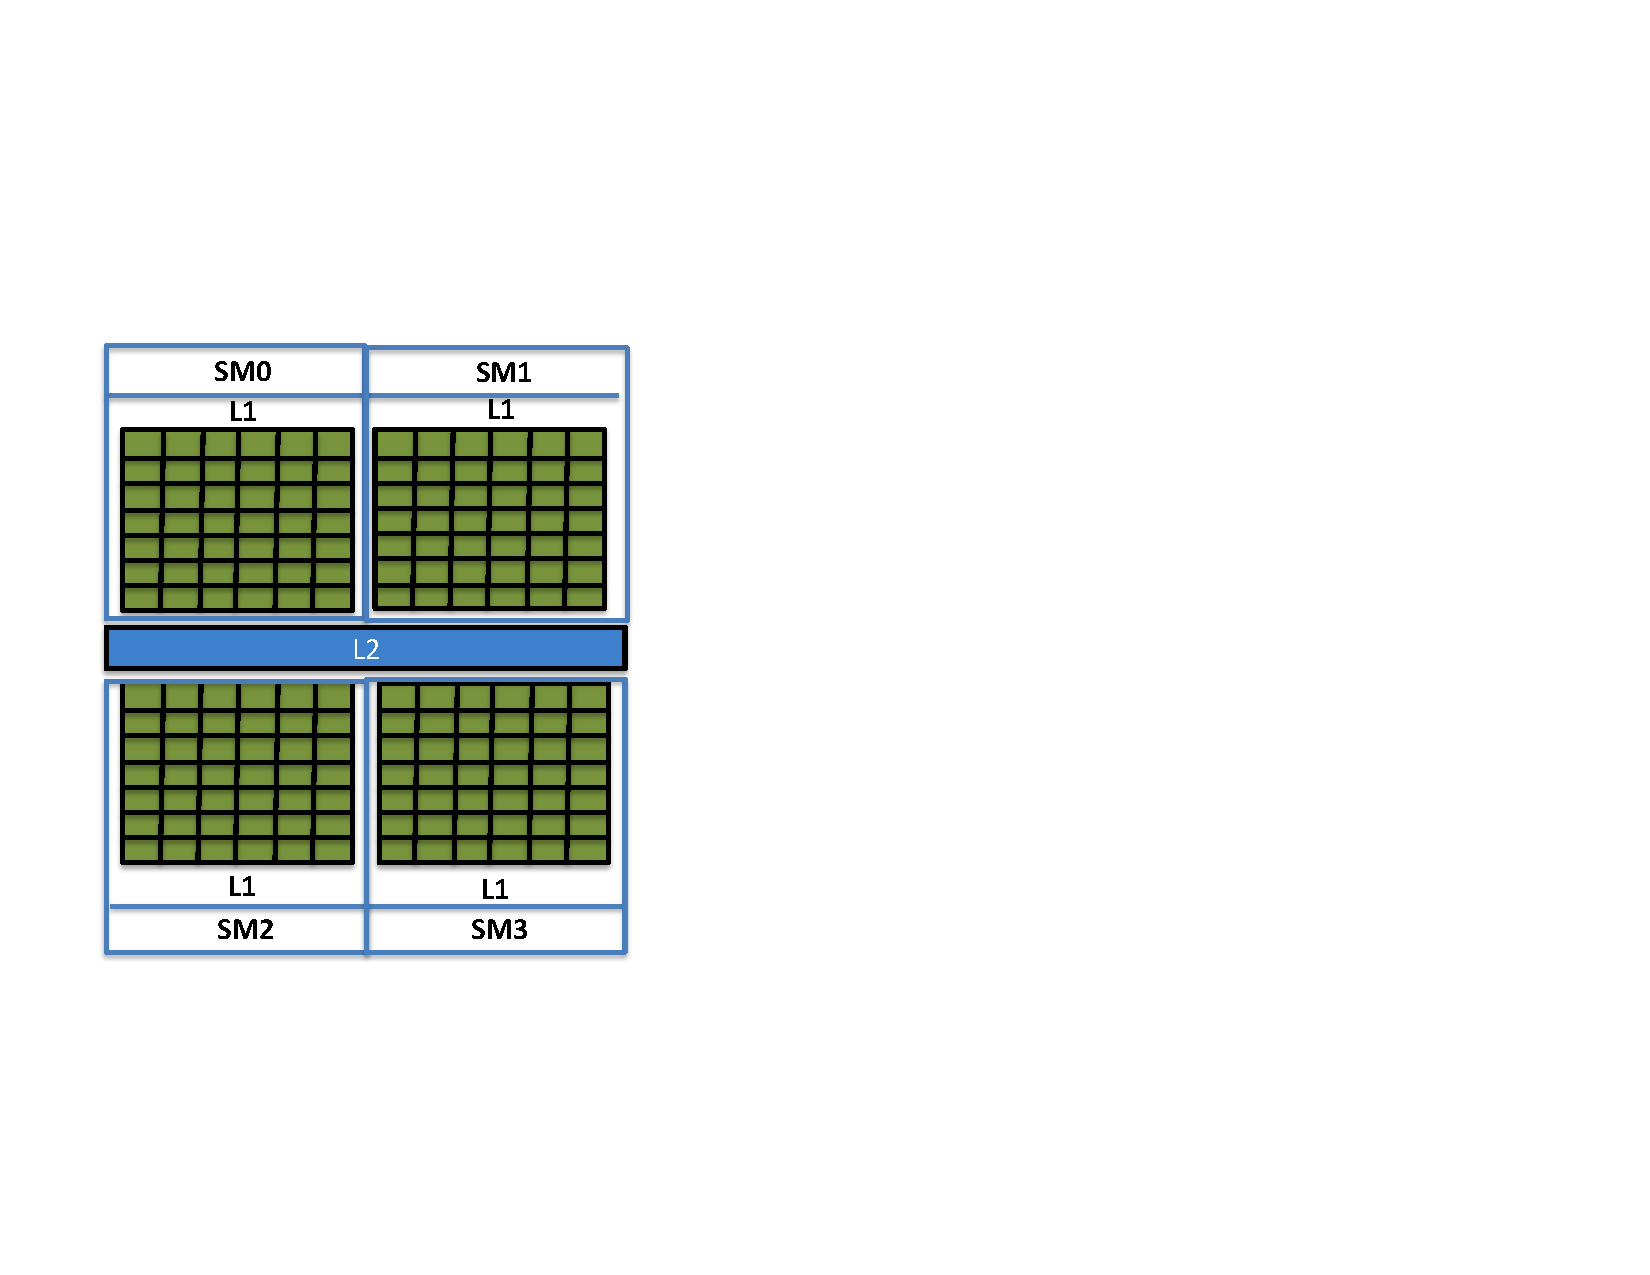
\includegraphics[width=\textwidth]{figures/SMs.pdf}
%\caption{A GPUs with 4 SMs}
%\label{SMs}
%\end{subfigure}
%\begin{subfigure}[b]{0.2\textwidth}
%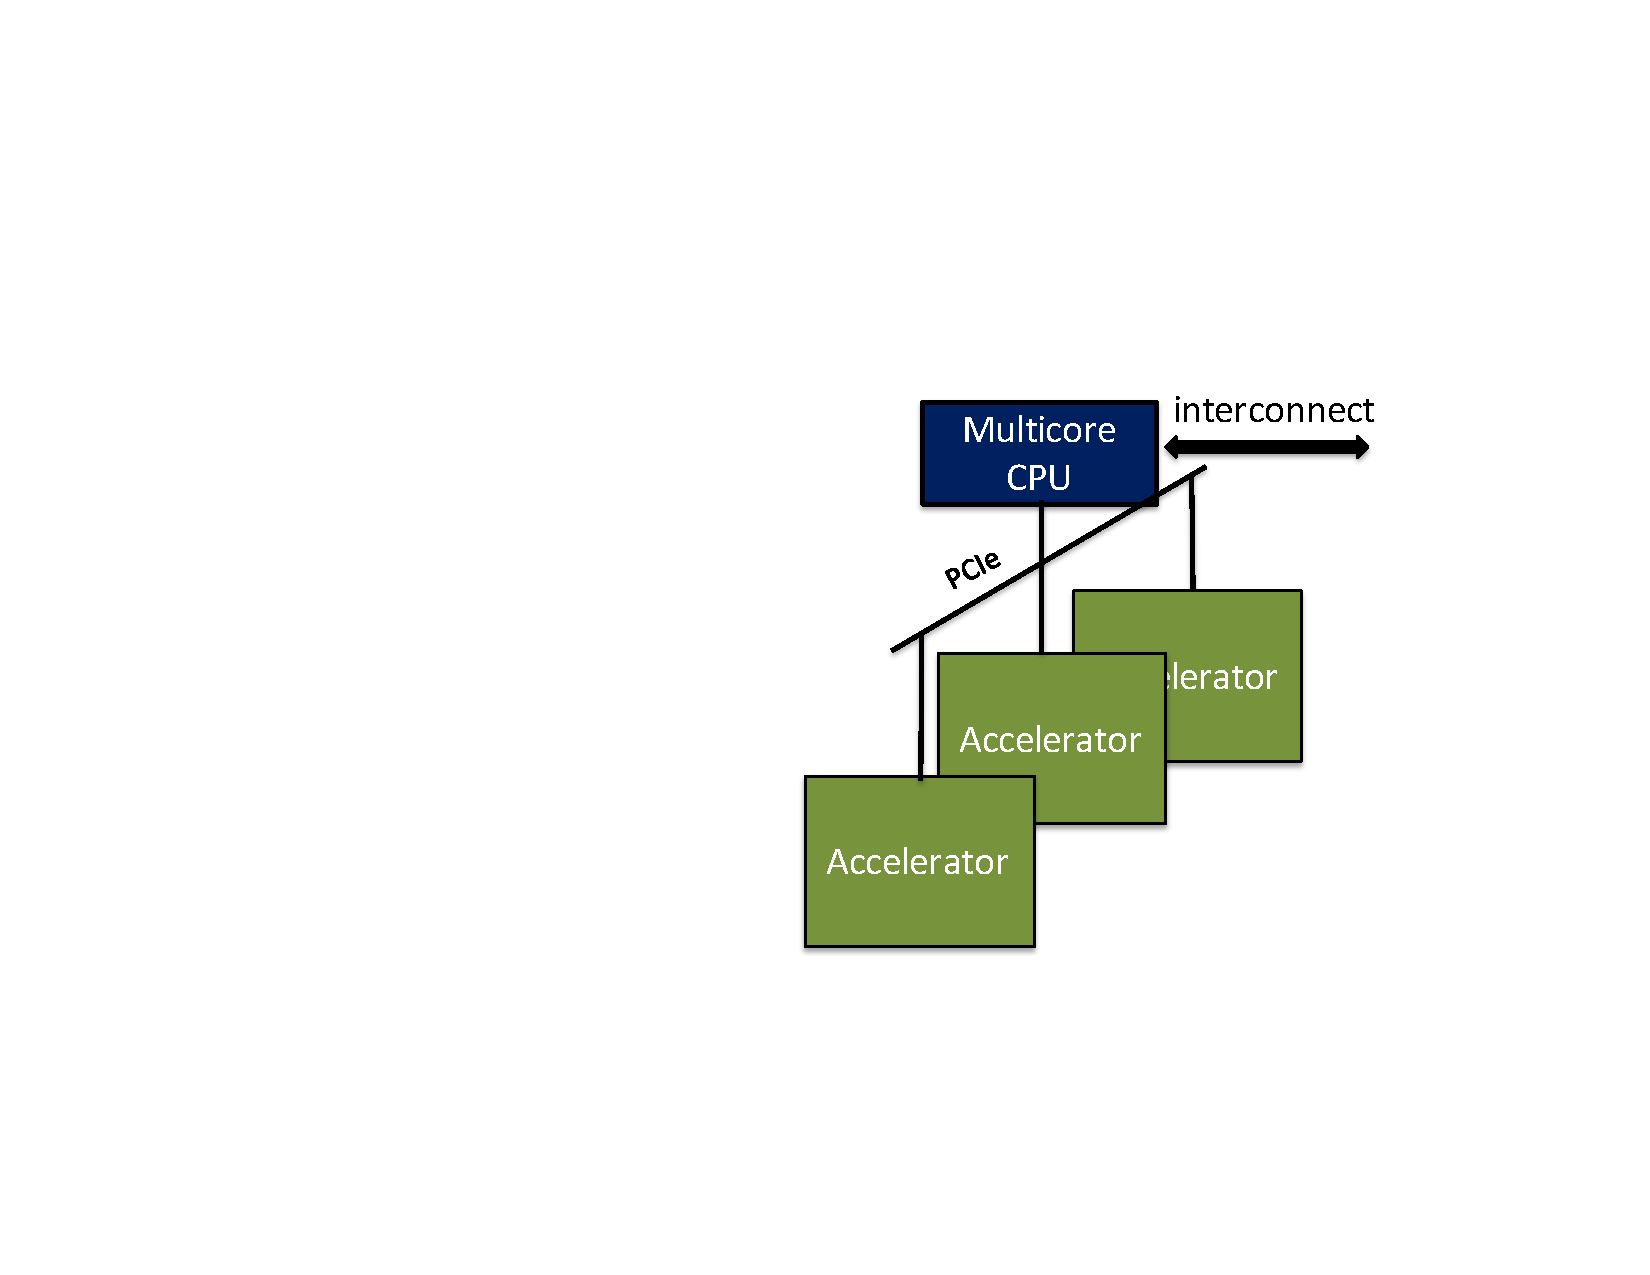
\includegraphics[width=\textwidth]{figures/host_accelerator.pdf}
%\caption{Host with accelerators}
%\label{hybrid}
%\end{subfigure}
%\caption{A hybrid node design}
%\label{fig:sysArch}
%\end{figure}


